\subsection{Theoretischer Aufbau der Messapparatur}
\label{sec:Versuchsaufbau}

\begin{figure}
    \centering
    \begin{subfigure}{0.48\textwidth}
        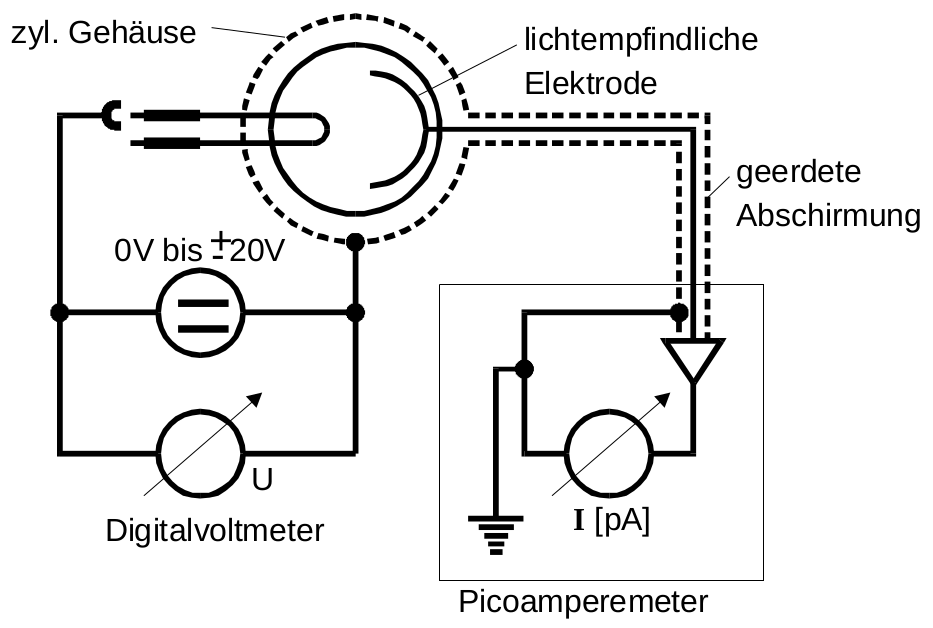
\includegraphics[width=\textwidth]{Bilder/schaltbild.png}
        \caption{Elektrisches Schaltbild der Photozelle \cite{Anleitung}.}
        \label{fig:schalte}
    \end{subfigure}
    \begin{subfigure}{0.48\textwidth}
        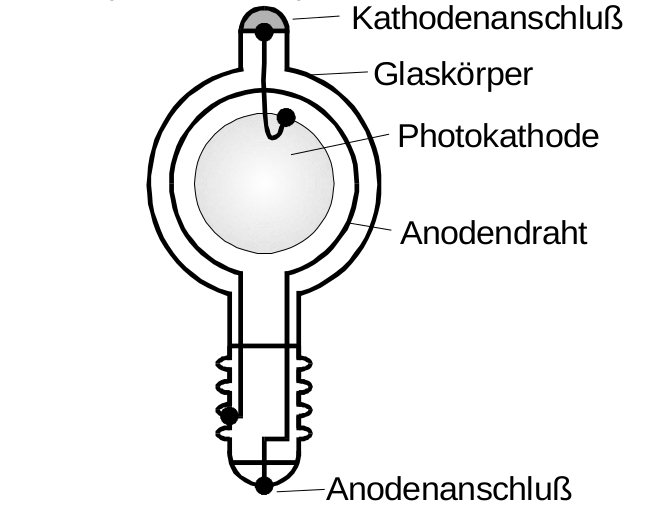
\includegraphics[width=\textwidth]{Bilder/aufbau_photozelle.png}
        \caption{Schematischer Aufbau einer Photozelle \cite{Anleitung}.}
        \label{fig:photozelle}
    \end{subfigure}
\end{figure}
Der prinzipielle Aufbau einer Photozelle ist in Abbildung \ref{fig:photozelle} dargestellt.
Diese besteht aus zwei Elektronen in einem evakuierten Glaskolben.\\ Eine der beiden Elektronen wird hierbei als Photokathode bezeichnet. Sie ist mit einer Metall- oder Legierungsschicht bedampft, welche vom einfallenden Licht bestrahlt werden kann.\\
Die Anode ist als Drahtring in einigen Millimetern Abstand zur Photokathode realisiert.
In Abbildung \ref{fig:schalte} ist der elektrische Schaltplan der Messapparatur dargestellt.\\
Zwischen Kathode und Anode befindet sich ein Digitalvoltmeter, sodass eine variable Spannung $U$ angelegt werden kann, durch die ein elektrisches Feld erzeugt werden kann, welches die Elektronen abbremst.\\
Mithilfe eines Picoamperemeters kann der zwischen Photokathode und Anode fließende Strom gemessen werden.\\
\begin{figure}
  \centering
  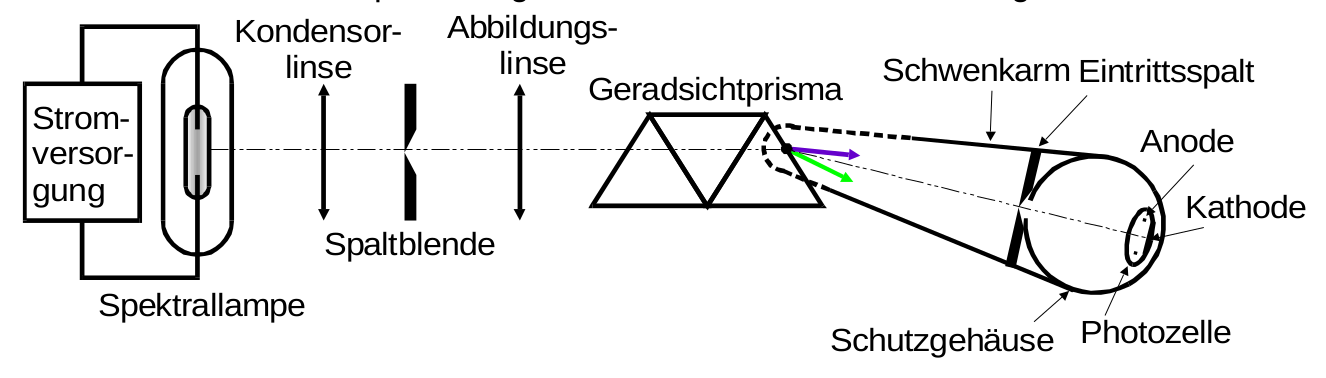
\includegraphics[width=0.98\textwidth]{Bilder/versuchsaufbau.png}
  \caption{Prinzipieller Aufbau der Messapparatur \cite{Anleitung}.}
  \label{fig:aufbau}
\end{figure}
In Abbildung \ref{fig:aufbau} ist der Aufbau der Messapparatur dargestellt.\\
Das Licht der Spektrallampe läuft zunächst durch eine Kondensorlinse. Diese dient dazu, einen möglichst großen Teil des Lichts der Spektrallampe in den Strahlengang der Versuchsapparatur zu fokussieren.\\
Daher wird die Kondensatorlinse nahe der Spektrallampe angebracht, sodass ein Bild mit möglichst großer Intensität an der Photolinse erzeugt werden kann.\\ Der Lichtstrahl läuft anschließend zunächst durch eine Spaltblende und wird anschließend mittels einer Abbildungslinse auf ein Geradsichtprisma geworfen. Das Geradsichtprisma spaltet das einfallende Licht in seine Spektralfarben auf.\\
Mithilfe eines Schwenkarms kann die Photozelle so positioniert werden, dass jeweils nur monochromatisches Licht, also nur das Bild in einer der Spektralfarben durch den Eintrittspalt auf die Photozelle fallen kann.
